\section{Introduction}
\label{sec:intro}

For many database users, writing database queries is a struggle. It is a
struggle because mastering a query language requires training. It is also a
struggle because it requires a precise and exhaustive knowledge of the
database. Users must know exactly which table to use, which columns to inspect
and which conditions to set. When users \emph{explore} their data, that is,
when they are interrogating it to discover its content, they do not have this
knowledge.

To address this problem, software editors and researchers have come up
\emph{natural language interfaces} to databases. The idea is to let users
interrogate their databases with plain English. It is then up to the system to
interpret the query and cast it in a form that the underlying data manager can
understand. This approach constitutes a huge leap forward, but it is not exempt
of drawbacks. For a start, it still assumes that they user has a specific query
in mind. Even if they do not know how to express this query SQL, they must have
some idea of which column to use. Furthermore, it only solves half  of the
problem: the users express their queries in SQL, but they still obtain their
results in tabular format. If the output contains a few tuples and a handful of
columns, this paradigm is ideal. But what if the users are interested in
broader queries?

A popular alternative is to use visual tools, such as Tableau. With these
packages, users can write queries with drag and drops and obtain their results
with visualizations. But this approach has its limits too. It does not solve
the starting point problem, as users still need to write a query. Furthermore,
visualizations are no panacea. Their main drawback come from the fact that they
attempt to show everything. Consequently, they require training (though mild),
attention, and they cannot scale beyond a few dozen variables.

In this paper, we introduce Clustine, the first conversational agent for data
exploration. Our system remains on two pillars. First, it uses natural language
during the whole exploration process. This means that it collects queries, but
also \emph{answers} in natural language. While several papers have studied the
first direction, little to none of them have tackled the reverse direction.
Second, our system is proactive: it makes suggestions, instead of collecting
queries passively. It is then up to the user to accept or reject these
suggestions.

This paper is an early-stage report: we present the main ideas behind Clustine
and present preliminary experiments to show that they are feasible.
Nevertheless, we will omit a few details and leave questions open for future
publications. This work is partly inspired by Blaeu, a system to explore data
with cluster analysis. The main difference is that Blaeu relies heavily on
visualizations and expert judgment.

\section{Overview}
\label{sec:overview}

Clustine has several advantages compared to visual tools such as Tableau. It is
proactive, in the sense that it suggests questions to the user. Also, its scope
is ever broader that that of Tableau: it can be used by users with no literacy
in data analysis, user who rely on audio (e.g., visually impaired users), and
it is generally well suited to educational contexts. But the strengths of our
method are also its weaknesses. As Clustine makes ``editorial choices'', it
omits potentially interesting information about the data. Furthermore, full
text is much less space efficient than charts. Therefore, Clustine is
conceptually, but also materially limited.

\section{Architecture}
\label{sec:architecture}

\section{Use Cases}
\label{sec:demo}

\begin{figure}[t]
  \centering
  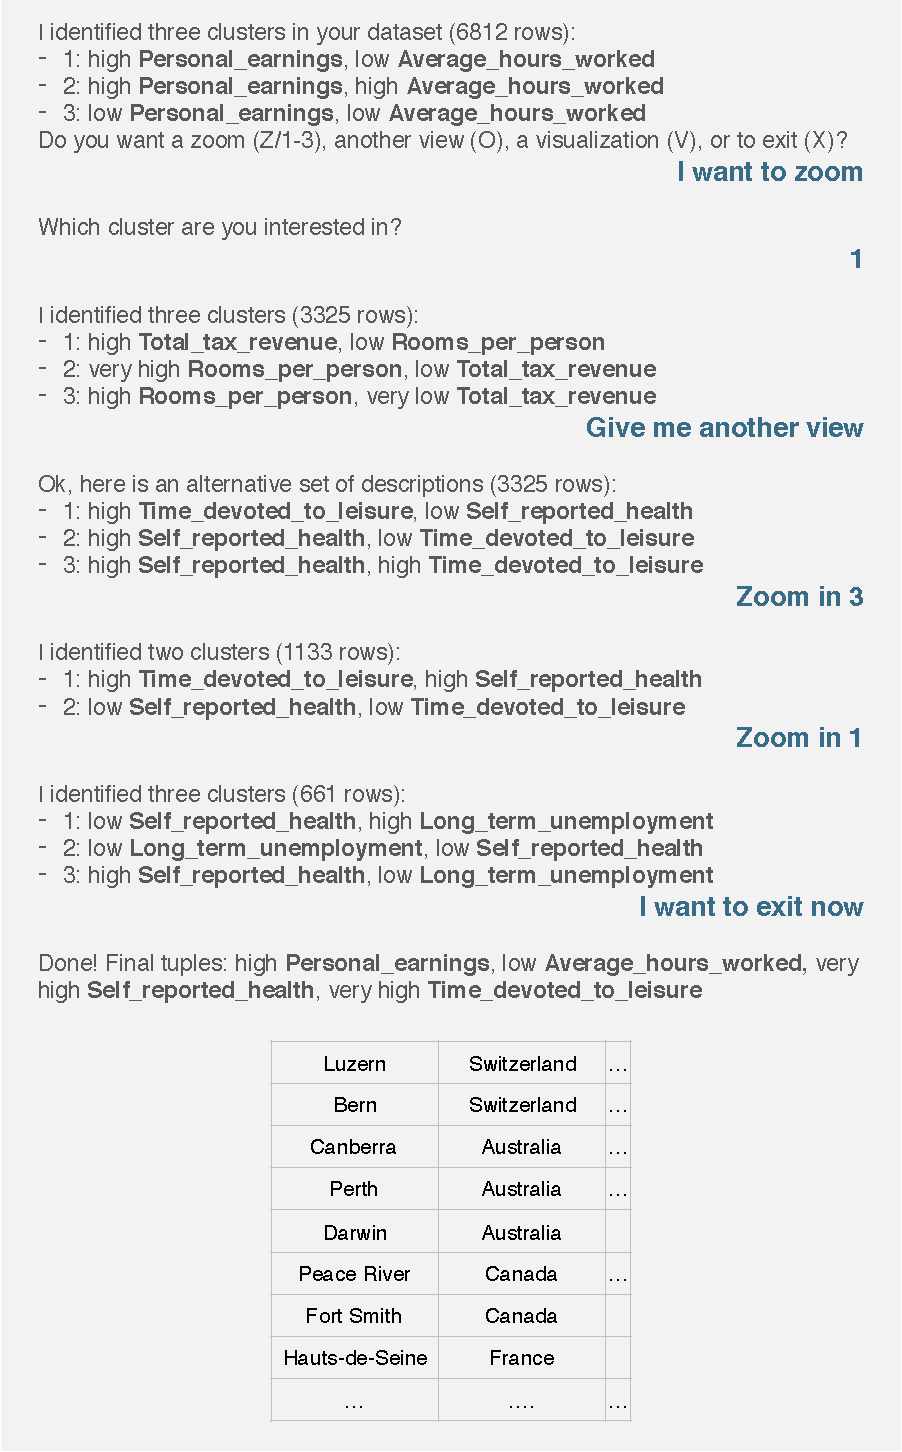
\includegraphics[width=\columnwidth]{Experiments/UseCaseFull}
  \caption{Demonstration 1: the OECD dataset.}
  \label{fig:UseCase1}
\end{figure}

\begin{figure}[t]
  \centering
  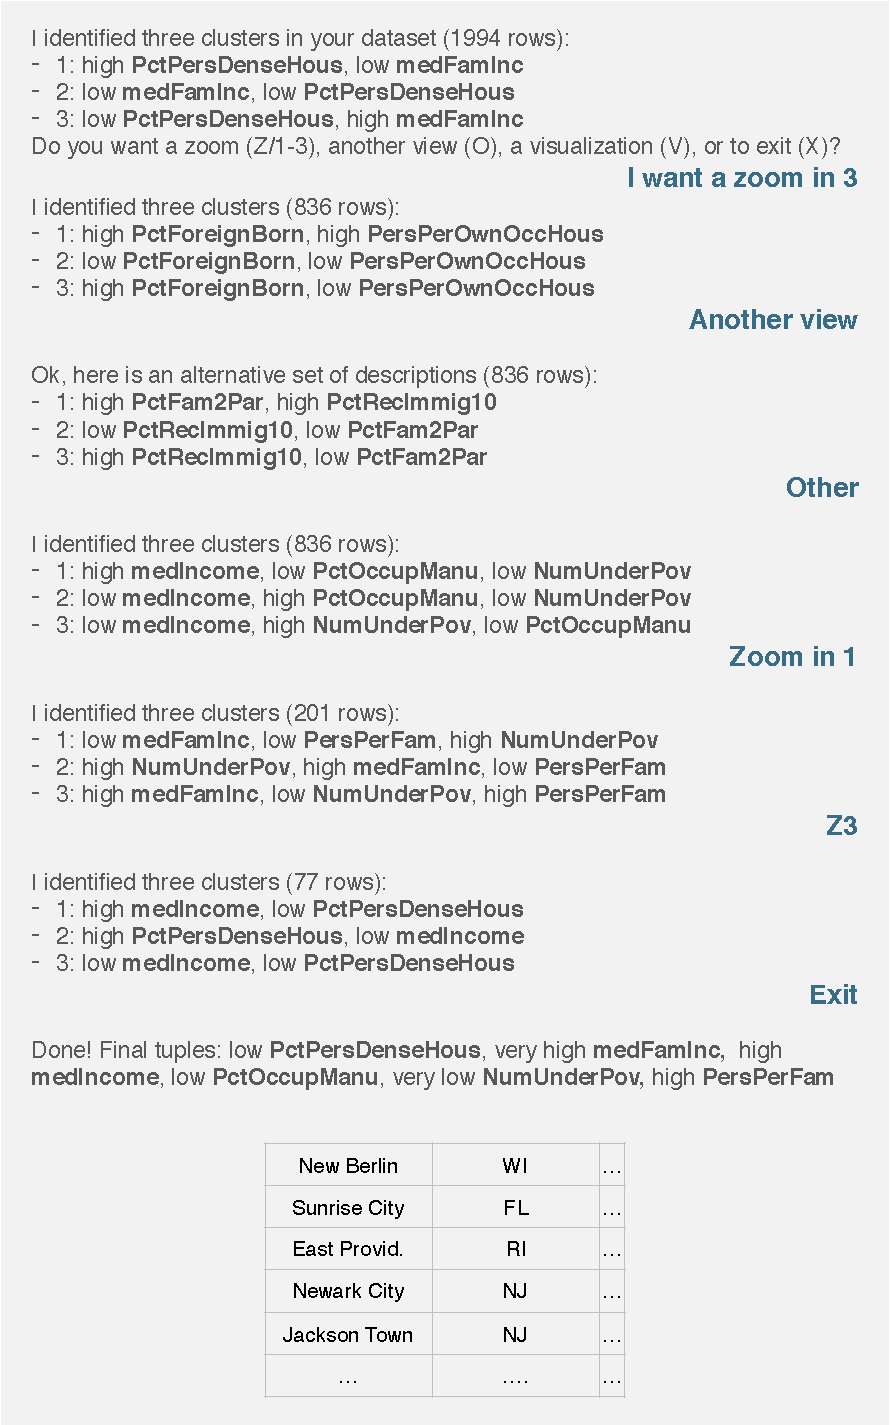
\includegraphics[width=\columnwidth]{Experiments/UseCase2}
  \caption{Demonstration 2: cities, crime and wealth in the US.}
  \label{fig:UseCase2}
\end{figure}

We now demonstrate Clustine with two real-life scenarios.  We start with the
full version of case we used as running example throughout the paper. Our
database comes from the OECD, an international economic
organization\footnote{http://stats.oecd.org/}. It describes economic, social
and well-being indicators for 2,180 regions in 31 countries, across three
years. In total it contains 6,823 rows and 519 columns. Our aim is the find the
countries with the ``best living conditions'', a purposely vague and subjective
task.

Figure~\ref{fig:UseCase1} presents our interaction with Clustine. We exploited
three of its five suggestions. First, we selected the regions with the highest
salaries and the lowest number of hours worked.  We then refined our selection
with attributes related to leisure time, health, then unemployment.  Observe
that Blaeu's second suggestion was irrelevant to us. We simply discarded it by
requesting a new view.

Our second scenario is based on the Crime and Communities dataset, from the UCI
repository\footnote{http://archive.ics.uci.edu/ml/}. The data contains 128
crime and socio-economic indicators for 1,994 US cities. Our aim is to find the
richest and safest communities. Figure~\ref{fig:UseCase2} represents Clustine's
suggestions and our answers. We see that the system manages to narrow our
selection to 77 rows in six questions. Also, the suggestions correspond to our
intuition. For instance, partitioning US cities on the variables Family Income
and Housing Density seemed natural to the author of this paper.  Finally, this
use case also highlights one limit of Clustine's model: it assumes that the
database's column names are self-explanatory. Unfortunately, this assumption
does not always hold. We leave the subsequent challenges for future work.

After each suggestion, Clustine gives the option to visualize the underlying
data. The aim is to let users perform ``sanity checks'' and obtain more
details. Figure~~\ref{fig:propvis} presents three of those visualizations - one
for the OECD dataset, two for the Crime dataset. In all cases, we observe that
the labels of the clusters do match their position in the attribute space.
 
\begin{figure*}
    \centering
    \begin{subfigure}[b]{0.3\textwidth}
        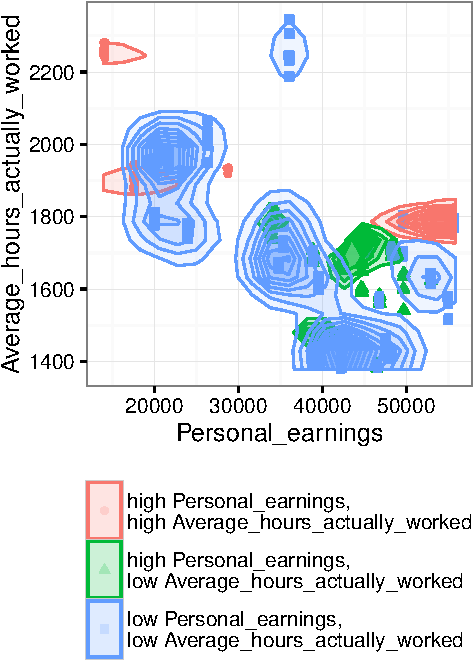
\includegraphics[width=\textwidth]{Experiments/CaseValidation1}
        \caption{OECD dataset, first suggestion.}
        \label{fig:validation1}
    \end{subfigure}
    ~
    \begin{subfigure}[b]{0.3\textwidth}
        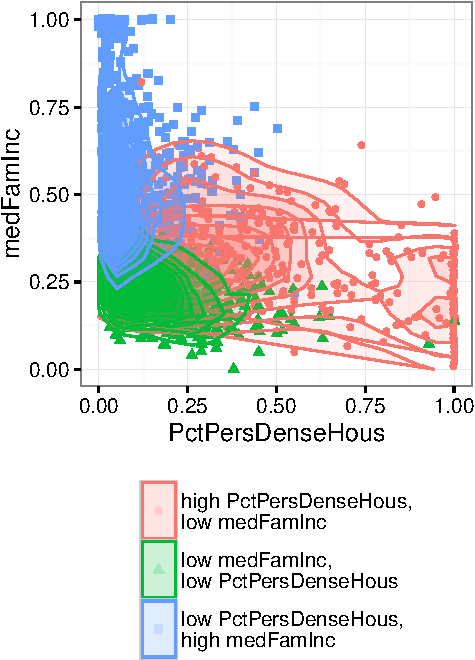
\includegraphics[width=\textwidth]{Experiments/Case2Validation1}
        \caption{Crime dataset, first suggestion.}
        \label{fig:validation2}
    \end{subfigure}
    ~
    \begin{subfigure}[b]{0.3\textwidth}
        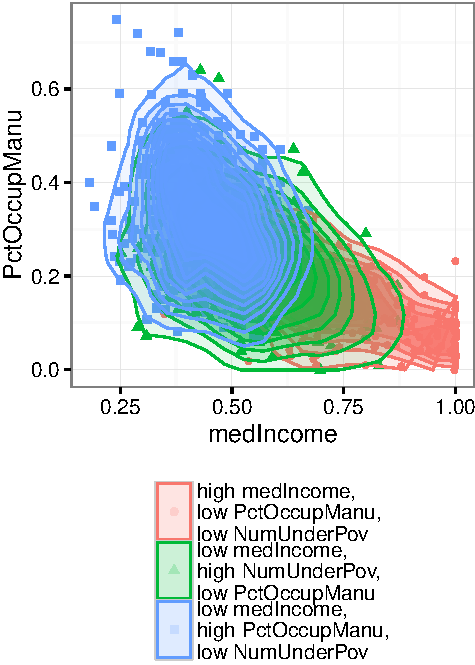
\includegraphics[width=\textwidth]{Experiments/Case2Validation8}
        \caption{A mouse}
        \label{fig:validation3}
    \end{subfigure}
    \caption{Two-dimension views of Clustine's suggestions.}\label{fig:propvis}
\end{figure*}


\section{Evaluation}
\label{sec:eval}
We now present our experimental results. To be efficient, Clustine must detect
meaningful clusters, describe them accurately and do so with a low latency.
The first aspect depends entirely on our choice of clustering algorithm.
Because we used EM, a well known algorithm~\cite{dempster1977maximum}, we will
not discuss it further in this paper. We will however present our evaluation of
Clustine's description engine. We will first focus on its accuracy, then on its
runtime.

\begin{table}[!t]
    \centering
    \small
    \begin{tabular}{r c c c c} 
        \hline
        Dataset & Columns & Rows\\
        \hline
        ShapeRecog & 16 & 180\\
        Glass & 8 & 226\\
        Vowels &  9&1,000  \\
        BreastCancer & 34 & 234\\
        PenDigits & 17 & 7,496\\
        MAGICTelescope & 11 & 19,022\\
        AdultCensus & 14 & 32,578\\
        LetterRecog & 16 & 20,000\\
        Crime & 128 & 1,996\\
        BankMarketing & 17 & 45,213\\
        Insurance & 86 & 5,900\\
        MuskMolecules & 167 & 6,600\\
        \hline
    \end{tabular}
    \caption{Characteristics of the datasets.}
    \label{tab:datasets}
\end{table}

\subsection{Experimental Setting}
All the experiments that follow are based on 12 datasets from the UCI
repository. We present their characteristics in Table~\ref{tab:datasets}. Our
experimental system is a MacBook Pro with an 2.6 GHz Intel Core i5 processor
and 8GB main memory. All our code is written in R, exploiting its native C
primitives for common operations (e.g., computing covariance matrices) and our
own C library for information theoretic operations (used in one of our
baselines).

In this section, we evaluate the quality of Clustine's column selection
algorithms. Our aim is to test whether the columns it choses are indeed
``descriptive'', that is, contain information about the structure of the data.
To do so, we use statistical classifiers. We first cluster each dataset with
the EM algorithm, as Clustine does. We materialize the result in a vector, in
which the $i^{\text{th}}$ component represent the cluster of the
$i^{\text{th}}$ tuple. Finally, we train a classifier to associate each its
tuple to its cluster, using only the columns provided by Clustine. If this
operation succeeds, then we can conclude that the columns are ``instructive'':
the projection contains all the information necessary to reconstitute the
clustering structure of the whole data. Oppositely, if the classifier fails,
then the chosen columns probably give a poor view of the data's overall
distribution.  Technically, we used a 5-Nearest Neighbors classifiers. We chose
it for its simplicity and efficiency. We measure the prediction accuracy with
the F1 score on 10-fold cross validation. Higher is better.

We benchmark Clustine's column selection algorithm against two standard feature
selection algorithm.  The first algorithm \texttt{Wrap-kNN} is a \emph{wrapper}
from the statistics literature~\cite{guyon2003introduction}. It builds sets of
columns greedily. It adds variables one after other, keeping at each stop those
that yield the best classification score. It stops when it obtained a view with
$D$ dimensions. We expect it to be slow but accurate, since it optimizes
exactly our metric. The algorithm \texttt{MutualInfo} computes the Mutual
Information (i.e., statistical dependency) between each variable and the
cluster assignment vector. It retains the top $D$ variables. We expect to be
fast, but less accurate than \texttt{Wrap-kNN}. We also added a random baseline
to ensure that the results are worth the effort.  By default, we set $D=3$. We
ran each experiment five times and averaged the results.

Compared to its competitors, Clustine has one qualitative advantage: it is a
``white box''. Since it exploits differences of means and variances, it
explains not only how much the clusters differ from one another but also
\emph{how} they differ - a property on which Clustine relies heavily to create
its explanations. Our hope is that it is also quantitatively better. Since we
target real-time interaction, our algorithms should be faster than all the
others, possibly at the cost of losses in accuracy.

\subsection{Accuracy of the Column Selection}
\label{sec:accuracy}
\begin{figure*}[t]
  \centering
  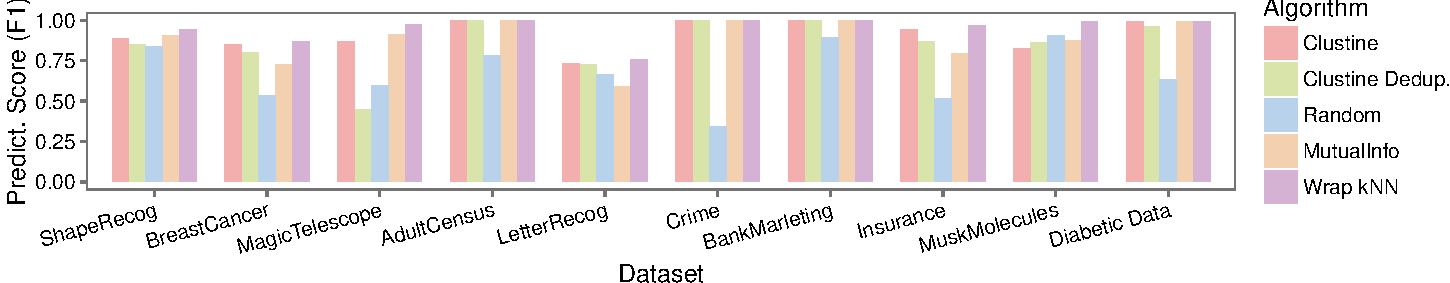
\includegraphics[width=\textwidth]{Experiments/F1_Scores}
  \caption{Accuracy of the variable selection algorithms. Higher is better.}\label{pic:accuracy}
\end{figure*}

Figure~\ref{pic:accuracy} presents the accuracy of our algorithms on each
dataset. We observe that \texttt{Wrap-kNN} dominates the scores in all cases.
It is then followed by \texttt{Clustine} and \texttt{Wrap-kNN}, with a weak
advantage for the former (\texttt{Clustine}'s score is equivalent or better
than \texttt{Wrap-kNN}'s in 8 cases out of 12). The random strategy comes
almost always last. In conclusion Clustine's accuracy is competitive: it is at
least as a good as a well established feature selection algorithm.

\subsection{Runtime of the Column Selection}
\label{sec:speed}

\begin{figure*}[t]
  \centering
  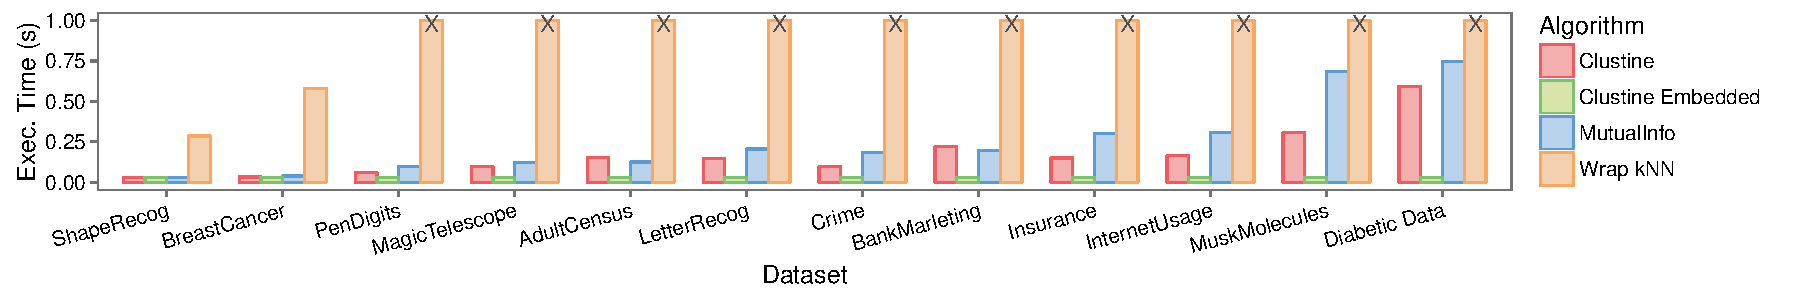
\includegraphics[width=\textwidth]{Experiments/Timings}
  \caption{Execution time of the variable selection algorithms. Lower is
  better. The cross indicates that the experiment exceeded 0.8 seconds.}
  \label{pic:runtime}
\end{figure*}

We present the results of our runtime experiments in Figure~\ref{pic:runtime}.
In all cases, \texttt{Clustine} is comparable to or much faster than
\texttt{MutualInfo}, an already fast algorithm. Since both algorithms scale
linearly with the number of rows and columns, the difference comes from the
constant factors. Computing and comparing means and variances appears faster
than estimating mutual informations (both operations were implemented in C).
We conclude that our algorithm is aggressively fast.

When we measured \texttt{Clustine}'s runtime, we accounted for the time
necessary to compute the mean and variance of each column. This measurement is
pessimistic. In practice, we obtain this information ``for free'' from the EM
algorithm, and therefore we can perform the column selection without even
reading the data. The bars associated with \texttt{Clustine Embedded} in
Figure~\ref{pic:runtime} show the runtime associated with the remaining
computations. We observe that they are almost negligible. Therefore, in
practice, the computational cost depends almost entirely on the EM algorithm.
We can consider the description itself as a minor overhead, demanding a few
milliseconds at worse.


\section{Related Work}
\label{sec:related}
See also \cite{li2014constructing}.

\section{Conclusion}
\label{sec:conclusion}
During the last few years, several companies have introduced virtual
assistants: Cortana, Siri, Google Voice. In this paper, we investigated how to
develop a similar system for data exploration.
